\documentclass[a4paper]{article}
\usepackage[UTF8]{ctex}
\usepackage{geometry}
\usepackage{graphicx}
\usepackage{url}
\usepackage{multirow}
\usepackage{array}
\usepackage{booktabs}
\usepackage{url}
\usepackage{enumitem}
\usepackage{graphicx}
\usepackage{float}
\usepackage{amssymb}
\usepackage{amsmath}
\usepackage{subfig}
\usepackage{longtable}
\usepackage{pifont}
\usepackage{color}

\allowdisplaybreaks

\geometry{a4paper, scale=0.78}

% \begin{figure}[H]
%     \centering
%     \includegraphics[width=.55\textwidth]{E.png}
%     \caption{矩阵与列向量的乘法}
%     \label{fig:my_label_1}
% \end{figure}

% \left\{
% \begin{array}{ll}
%       x+2x+z=2 & \\
%       3x+8y+z=12 & \\
%       4y+z=2
% \end{array}
% \right.

% \begin{enumerate}[itemindent = 1em, itemsep = 0.4pt, parsep=0.5pt, topsep = 0.5pt]

% \end{enumerate}

%\stackrel{a}{\longrightarrow}

%\underbrace{}_{} %下括号

%\tableofcontents %目录,并且目录页不记录页码
% \tableofcontents
% \newpage
% \setcounter{page}{1} %new page
% \clearpage

\title{Gaussian Network}
\author{Chen Gong}
\date{26 February 2020}

\begin{document}
\maketitle
%\pagestyle{empty}
\tableofcontents
\newpage
%\pagestyle{fancy}
\setcounter{page}{1} %new page
\clearpage
这小节,我们主要讲解的是高斯网络的结构背景,模型的基本概念。根据有向图和无向图,我们可以将高斯网络分成高斯贝叶斯网络和高斯马尔可夫网络。
\section{Background}
概率图模型(Probability Graphic Model),我们之前学习的是贝叶斯网络和马尔可夫随机场,之前学习的概率图中每个节点都是离散随机变量。所以根据图是有向图还是无向图,我们可以将概率图模型分成贝叶斯网络(Bayesian Network)和马尔可夫随机场(Markov Random Field)。

而如果概率图中每个节点都是一维连续随机变量,根据图是有向图还是无向图,可以被分为高斯贝叶斯网络(Gaussian Bayesian Network)和高斯马尔可夫随机场(Gaussian Markov Random Field)。
\subsection{高斯网络概念}
假设高斯马尔可夫随机场的概率图模型如下所示:
\begin{figure}[H]
    \centering
    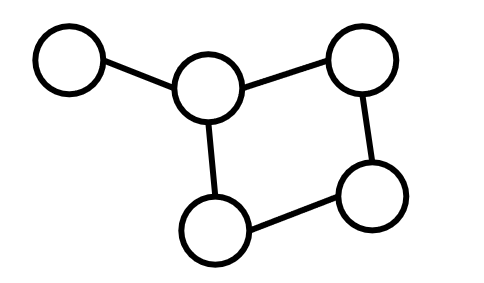
\includegraphics[width=.4\textwidth]{微信图片_20200226164330.png}
    \caption{高斯马尔可夫随机场的概率图模型}
    \label{fig:my_label_1}
\end{figure}
每一个节点都是一个一维随机变量,每一个节点$x_i \sim \mathcal{N}(\mu_i,\Sigma_i)$,而所有的节点构成的集合:$\mathcal{X}=(x_1,x_2,\cdots,x_p)^T$。多维变量的高斯分布为:
\begin{equation}
    P(X) = \frac{1}{(2\pi)^{\frac{p}{2}}|\Sigma|^{\frac{1}{2}}} \exp \left\{ -\frac{1}{2} (X-\mu)^T\Sigma^{-1}(X-\mu) \right\}
\end{equation}
所以,\textbf{一个高斯网络就可以映射为一个高维高斯分布}。而协方差矩阵$\Sigma$实际就反映了变量之间的联系。由于高斯分布的自共轭性,单个变量和整个高斯网络都是符合高斯分布的。

协方差矩阵为:
\begin{equation}
    \Sigma = (\sigma_{ij}) = 
    \begin{bmatrix}
    \sigma_{11} & \sigma_{12} & \cdots &\sigma_{1p} \\
    \sigma_{21} & \sigma_{22} & \cdots &\sigma_{2p} \\
    \vdots & \vdots & \ddots & \vdots \\
    \sigma_{p1} & \sigma_{p2} & \cdots &\sigma_{pp} \\
    \end{bmatrix}_{p\times p}
\end{equation}
而协方差矩阵描述的就是两个变量之间关系,当$\sigma_{ij}=0$,就等价于$x_i \perp x_j$。整个是绝对独立或者称之为边缘独立,而在我们概率图模型中往往研究的是条件独立,$x_A \perp x_B | x_C$($x_A,x_B,x_C$都是节点的集合)。我们研究条件独立性实际上是为了简化计算,因为完全图的复杂度实在是太高了。

我们定义信息矩阵(Information Matrix)或者也被称为精度矩阵(Precision Matrix)为:
\begin{equation}
    \Lambda = \Sigma^{-1} = \begin{bmatrix}
    \lambda_{11} & \lambda_{12} & \cdots &\lambda_{1p} \\
    \lambda_{21} & \lambda_{22} & \cdots &\lambda_{2p} \\
    \vdots & \vdots & \ddots & \vdots \\
    \lambda_{p1} & \lambda_{p2} & \cdots &\lambda_{pp} \\
    \end{bmatrix}_{p\times p}
\end{equation}
当$\lambda_{ij}=0$就意味着$x_i\perp x_j |-\{x_i,x_j \}$这就可以用来表示条件概率了。这也是信息矩阵的微妙之处,至于为什么我们相信大部分同学都是一脸懵逼,这里会在后面进行描述。

\subsection{小结}
Gaussian Network是连续型的概率图模型,一个高斯网络实际上可以看成是一个高维高斯分布。协方差矩阵中可以反映完全独立性,而精度矩阵中可以反映条件独立性,也就是在其他所有节点已知的情况下,两个节点之间的独立性。下面我们要分别介绍Gaussian Bayesian Network和Gaussian Markov Random Field。

\section{Gaussian Bayesian Network}
在连续型的Probability Graphic Model中,有向图,被我们称之为Gaussian Bayesian Network。假设概率图中一共有$p$个节点,根据我们之前学习的贝叶斯网络的因子分析法,可以得到:
\begin{equation}
    P(X) = \prod_{i=1}^p P(x_i|x_{\mathrm{pa}(i)})
\end{equation}
$\mathrm{pa}(i)$是一个集合,代表$x_i$节点的父亲节点集合。

{\color{red} GBN is based on Linear Gaussian Model}。GBN是一个global的概念,代表的是整个高斯网络,也就是$X$之间的高维高斯分布。而Linear Gaussian Model指的是local的模型,也就是局部父亲节点与孩子节点之间的关系是符合高斯线性模型的。

我们看看标准的线性高斯模型:
\begin{equation}
    \left\{
    \begin{array}{ll}
      P(x) = \mathcal{N}(x|\mu_x,\Sigma_x) & \\
      P(y|x) = \mathcal{N}(y|Ax+b,\Sigma_y) & \\
    \end{array}
    \right.
\end{equation}
线性就体现在了$y$与$x$之间的关系。

\subsection{Kalman Filter回顾}
我们以HMM为例,概率图模型如下所示:
\begin{figure}[H]
    \centering
    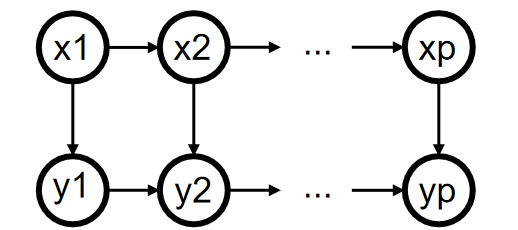
\includegraphics[width=.38\textwidth]{微信图片_20200226202312.png}
    \caption{Kalman Filter的概率图模型}
    \label{fig:my_label_1}
\end{figure}
Kalman Filter是用来解决HMM问题中的Filter问题,也被称之为线性高斯系统,线性主要体现在下面两个地方:
\begin{equation}
    \left\{
    \begin{array}{ll}
      P(x_t|x_{t-1}) = \mathcal{N}(x_t|Ax_{t-1}+B,Q) & \\
      P(y_t|x_t) = \mathcal{N}(y_t|Cx_t+D,R) & \\
    \end{array}
    \right.
\end{equation}
变量之间的线性关系即为:
\begin{equation}
    \left\{
    \begin{array}{ll}
      x_t = Ax_{t-1} + B + \epsilon & \epsilon\sim \mathcal{N}(0,Q) \\
      y_t = Cx_{t} + D + \delta & \delta \sim \mathcal{N}(0,R) \\
    \end{array}
    \right.
\end{equation}
这就是Kalman Filter的Representation Model,也就是一种特殊的Gaussian Bayesian Model。

\subsection{Gaussian Bayesian Model详解}
下面我以如下所示的Gaussian Bayesian Model为例:
\begin{figure}[H]
    \centering
    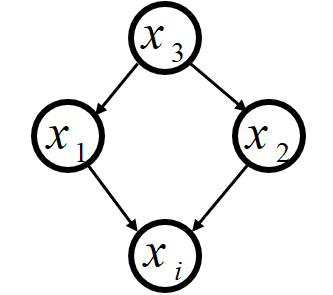
\includegraphics[width=.28\textwidth]{微信图片_20200226204441.png}
    \caption{Gaussian Bayesian Model的概率图模型}
    \label{fig:my_label_1}
\end{figure}
很显然$x_{\mathrm{pa}(i)}=\{x_1,x_2\}$。根据因子分解法,我们可以得到:
\begin{equation}
    P(X) = \prod_{i=1}^p P(x_i|x_{\mathrm{pa}(i)})
\end{equation}
我们将$x_{\mathrm{pa}(i)}$写成向量形式,所以$x_{\mathrm{pa}(i)} = (x_1,x_2,\cdots,x_k)$。根据父子节点之间的线性关系,我们可以得到:
\begin{equation}
    P(x_i|x_{\mathrm{pa}(i)}) = \mathcal{N}(x_i|\mu_i + w^T_ix_{\mathrm{pa}(i)}, \sigma_i^2 )
\end{equation}
其中,$x_i$是一维变量,实际上我们可以看\textbf{成$x_i$就是它的父亲节点的线性组合},所以说Guassian Network是基于局部模型,局部模式是一个Linear Gaussian Model,为了清楚表示可以写为:
\begin{equation}
    x_i = \mu_i + \sum_{j \in x_{\mathrm{pa}(i)}} w_{ij}\cdot(x_j-\mu_j) + \sigma_i \cdot \xi_i
\end{equation}
这里有的小伙伴可能会有点懵逼了,实际上我们将这个$x_j$写成$(x_j-\mu_j)$,是为了使其进行归一化,使均值等于0,以0为中心,便于对learning的运算。而$\xi_i \sim \mathcal{N}(0,1)$,我们知道$\sigma_i \cdot \xi_i$的方差还是为$\sigma^2$,而乘上一个随机变量是使$x_i$变成一个随机变量。而为了统一结构,我们将其写为:
\begin{equation}
    x_i - \mu_i = \sum_{j \in x_{\mathrm{pa}(i)}} w_{ij}\cdot(x_j-\mu_j) + \sigma_i \cdot \xi_i
\end{equation}
很显然,这就是一种线性组合。从全局角度看就是Gaussian Network,从局部角度来看就是一个Linear Gaussian Model。

\subsection{Gaussian Bayesian Model的矩阵表达形式}
假如,高斯网络中有p个节点,各个节点变量组成的集合为:
$$
X=(x_1,x_2,\cdots,x_p)^T
$$

相应每个节点的均值为:
$$
\mu=(\mu_1,\mu_2,\cdots,\mu_p)^T
$$

每个节点对应的一个$\mathcal{N}(0,1)$的随机变量为:
$$
\xi=(\xi_1,\xi_2,\cdots,\xi_p)^T
$$

节点与节点之间的权重组成了一个矩阵为:
$$
W = [w_{ij}]_{p\times p}
$$

而$S$为$\sigma_{i}$组成一个对角矩阵:
$$
S = \mathrm{diag}(\sigma_i)_{p \times p}
$$

所以,我们就可以得到Gaussian Linear Representation的向量表达形式为:
\begin{equation}
    X-\mu = W(X-\mu) + S\cdot \xi
\end{equation}
化简就可以得到:
\begin{equation}
    X - \mu = (I-W)^{-1} S\cdot \xi
\end{equation}
当然我们都假设这里都是可逆的。因为$X\sim \mathcal{N}(\mu,\Sigma)$,我们把变量看成$X-\mu$,所以重点要计算的就是$\Sigma$了。
$$
\Sigma = \mathrm{cov}(X) = \mathrm{cov}(X-\mu) = \mathrm{cov}((I-W)^{-1} S\cdot \xi) 
$$
$$
\mathrm{cov}((I-W)^{-1} S\cdot \xi) = ((I-W)^{-1} S)^T((I-W)^{-1} S)\mathrm{cov}(\xi) = ((I-W)^{-1} S)^T((I-W)^{-1} S)
$$
因为这里的$(I-W)^{-1} S$是一个确定的常数。

\subsection{小结}
在这一小节中,我们主要研究了连续随机变量的有向图,为Gaussian Bayesian Model,我们主要研究的是模型的表达形式,包括向量表达形式。最后,老师在求协方差矩阵的时候,没有求完,我觉得比较简单就顺手写了。\textbf{高斯贝叶斯模型,全局是多维高斯分布,局部是线性高斯模型。}

\section{Gaussian Markov Random Field}
这小节我们要介绍的连续变量的无向图结构,高斯马尔可夫随机场(Gaussian Markov Random Field)。多维高斯分布的概率密度函数如下所示:
\begin{equation}
    P(X) = \frac{1}{(2\pi)^{\frac{p}{2}}|\Sigma|^{\frac{1}{2}}} \exp \left\{ -\frac{1}{2} (X-\mu)^T\Sigma^{-1}(X-\mu) \right\}
\end{equation}

假设现有一个Gaussian Markov Random Field如下图所示:
\begin{figure}[H]
    \centering
    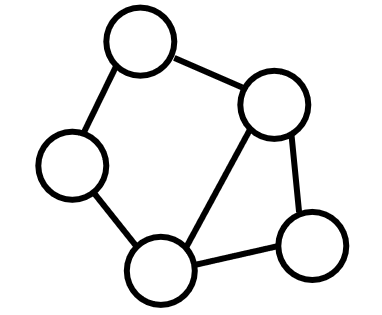
\includegraphics[width=.28\textwidth]{微信图片_20200226224151.png}
    \caption{Gaussian Markov Random Field的概率图模型}
    \label{fig:my_label_1}
\end{figure}

\subsection{Gaussian Markov Random Field的概率计算}
之前,我们使用了最大团的势函数的乘积来计算随机变量的概率。这里成对Markov性质,我们使用另一种表达方式,更适合对此问题的分析。我们假设模型中有$p$个节点,那么概率表达如下所示:
\begin{equation}
    P(X) = \frac{1}{Z} \prod_{i=1}^p \phi(x_i) \cdot \prod_{i,j\in X} \phi_{ij}(x_i,x_j)
\end{equation}
其中$\phi(x_i)$表示的是一个点的势函数,被称为node potential;而$\phi_{ij}(x_i,x_j)$表示的是一条边的势函数,被称为edge potential。令$\Sigma^{-1}=\Lambda$,下面我来计算$P(X)$的表达形式,为了清晰的分析,我们只考虑和$X$相关的部分。
\begin{equation}
    \begin{split}
        P(X) & \propto \exp \left\{ -\frac{1}{2}(X-\mu)^T \Sigma^{-1} (X-\mu) \right\} \\
        & = \exp \left\{ -\frac{1}{2}(X^T\Lambda - \mu^T \Lambda ) (X-\mu) \right\} \\
        & = \exp \left\{ -\frac{1}{2}(X^T\Lambda X - X^T \Lambda \mu - \mu^T\Lambda X + \mu^T \Lambda \mu \right\} \\
    \end{split}
\end{equation}
其中,$X$和$\mu$是$p \times 1$的矩阵,$\Lambda$是$p \times p$的矩阵。所以,$X^T \Lambda \mu$和$\mu^T\Lambda X$都是一维实数,且$X^T \Lambda \mu =\mu^T\Lambda X $(这还无法理解就自己拆开算一下吧)。
$$
P(X) \propto \exp \left\{ -\frac{1}{2}(X^T\Lambda X - 2 \mu^T\Lambda X + \mu^T \Lambda \mu ) \right\}
$$
最后一项$\mu^T \Lambda \mu$与$X$无关,所以
$$
    P(X) \propto \exp \left\{ -\frac{1}{2}(X^T\Lambda X - 2 \mu^T\Lambda X ) \right\} = \exp \left\{ -\frac{1}{2} X^T\Lambda X + \mu^T\Lambda X  \right\}
$$
又因为,$\Lambda$是对称矩阵,所以$(\mu^T\Lambda)^T = (\Lambda \mu) $,所以:
\begin{equation}
    P(X) \propto \exp \left\{ -\frac{1}{2} X^T\Lambda X + (\Lambda \mu)^T X \right\}
\end{equation}

其中$X^T\Lambda X$为二次项,$(\Lambda \mu)^T X$为一次性,其中$\Lambda$为Precision Matrix,$\Lambda \mu$为Potential Matrix。

\subsection{Gaussian Markov Random Field次项分析}
我们来从(17)中提取一下和$x_i$相关的项,提取的方法直接寻找相关项就行:
\begin{equation}
    x_i:\ -\frac{1}{2} x_i^2 \lambda_{ii} + h_ix_i
\end{equation}
其中,$h_i$为一个$p$维的向量。

接着从(17)提取和$x_i$和$x_j$的相关项:
\begin{equation}
    x_i,x_j:\ -\frac{1}{2} (\lambda_{ij}x_ix_j + \lambda_{ji}x_jx_i) = -\lambda_{ij}x_ix_j 
\end{equation}
因为,$\Lambda$是对称矩阵。

当$\lambda_{ij}x_ix_j=0$,就意味着边上的势函数就等于0,就意味着两个点之间是没有边是直接相连的。\textbf{因为没有边直接向量,那么在其他点都观察到的情况下,$x_i$和$x_j$之间是相互独立的。}所以,$\lambda_{ij}x_ix_j=0$就蕴涵着$x_i\perp x_j|-\{x_i,x_j\}$,这实际上非常的巧妙。所以,通过上述的分析,我们就成功的把多维高斯分布和一个无向图结合在了一起。所以,我们对$P(X)$进行研究的目的就是想知道,多维高斯模型和无向图之间的关系。\textbf{通过$\Lambda$矩阵做到了一个结合,这也就是我们在公式(3)下方给出的结论的原因。}

我们可以看到,\textbf{在对Gaussian Distribution的参数进行学习的过程中,我们不仅可以学习到了参数,也同时根据$\Lambda$的也就可以学习到结构($\lambda_{ij}x_ix_j=0 \Longleftrightarrow x_i\perp x_j|-\{x_i,x_j\}$ )。}因为高斯分布和高斯马尔可夫场的巧妙联系,在学习的过程中参数和结构都有考虑,这样的做法是非常棒的。

\subsection{小结}
本小节,最重要的就是三点,这里总结一下:
\begin{itemize}
    \item $x_i \perp x_j$中,$\Sigma = [\sigma_{ij}]$,$x_i \perp x_j \Longleftrightarrow \sigma_{ij} = 0$,也就是边缘独立,或者说是完全独立。
    \item $x_i \perp x_j|-{x_i,x_j}$中。$\Lambda = \Sigma^{-1} = [\lambda_{ij}]$,$x_i \perp x_j|-{x_i,x_j} \Longleftrightarrow \lambda_{ij}=0 $,这就是条件独立的特点。
    \item $\forall x$,$P(x_i|-{x_i})\sim \mathcal{N}(\sum_{i\neq j}\frac{\lambda_{ij}}{\lambda_{ii}}x_j,\lambda_{ii}^{-1}(\sigma_{ii}) )$,根据这个公式,我们可以深刻的体会到$x_i$可以看做其他与其相连的$x_j$的线性组合。这个公式是怎么算来的呢?实际上思路很简单,
    $$X = \begin{bmatrix} x_i \\ -\{ x_i\} \end{bmatrix}=\begin{bmatrix} x_a \\ { x_b} \end{bmatrix}$$
    而如果在知道高斯分布联合概率分布的情况下,求解条件概率分布是有系统的推导方法的。这里就不推了,有兴趣的同学自己请查阅之前讲到的“[机器学习基础 02]白板推导 数学基础”,\textbf{并且参考up主的思路,或者PRML的第二章P85,条件高斯分布。有详细的推导。}
\end{itemize}

\section{总结(Conclusion)}
本小节主要介绍了连续变量的概率图模型,高斯网络,根据有向图和无向图,可以分为高斯贝叶斯网络和高斯马尔可夫网络。我觉得高斯贝叶斯的主要思路是考虑整体高斯网络和局部线性高斯模型之间的联系,高斯马尔可夫的主要思路是考虑网络和联合概率密度函数之间的关系。他们都是将复杂的模型进行简化,迁移到简单的模型中去解决。但是,我们只学习了模型的建立和结构特点,并没有学习根据这个结构使用数据来求得参数的过程,相关研究领域的同学可以自行研究,如果不是要用到这个,基本就可以到此为止了。小编的主要研究方向是强化学习,此处就不再做更多的解释。




\end{document}
